\documentclass[11pt]{article}
%
%.....Packages used
%
\usepackage{graphicx,textcomp}
%\usepackage[sort,compress,colon,square,numbers]{natbib}
\usepackage[square,sort,comma,numbers]{natbib}
\bibliographystyle{plainnat}
\usepackage{url}

\usepackage{amsmath,amsfonts,amsthm,eucal}
\usepackage{enumerate}
\usepackage[letterpaper,margin=1in]{geometry}
\usepackage{setspace}
\usepackage{float,color}
\usepackage[colorlinks,linkcolor=blue,citecolor=blue]{hyperref}
\usepackage{multirow}
\usepackage{authblk}
%\usepackage{pdfsync}
%
%.....User defined commands and environments
%
\newcommand{\tensor}[1]{\ensuremath{\boldsymbol{#1}}}
\newcommand{\jump}[1]{\lbrack\!\lbrack #1 \rbrack\!\rbrack}
\newcommand{\alert}[1]{\textcolor{red}{#1}}
\newcommand{\avg}[1]{\left<#1\right>}
\DeclareMathOperator{\grad}{\nabla^{\tensor x}}
\DeclareMathOperator{\diver}{\nabla^{\tensor x}\cdot}
\DeclareMathOperator{\lap}{\Delta^{\tensor x}}
\DeclareMathOperator{\Grad}{\nabla^{\tensor X}}
\DeclareMathOperator{\Diver}{\nabla^{\tensor X}\cdot}
\DeclareMathOperator{\sym}{sym}
\DeclareMathOperator{\skw}{skw}
\DeclareMathOperator{\tr}{tr}
\DeclareMathOperator{\dev}{dev}
\DeclareMathOperator{\meas}{meas}
\newtheorem{prop}{Proposition}
\theoremstyle{remark}
\newtheorem{rmk}{Remark}
\floatstyle{plaintop}
\newfloat{boxes}{tbp}{lop}
\floatname{boxes}{Box}

\doublespacing
 \usepackage{lineno}
%  \linenumbers
%
%.....Begin Document
%

\title{Notes on Linear Regression}
\author[1]{Keng-Wit Lim\thanks{kengwit@gmail.com}}
\affil[1]{XXXX Los Angeles, CA, USA}

\renewcommand\Authands{ and }

\begin{document}

\maketitle
%\begin{center}
%\LARGE{Hardening Soil Model}\\
%\begin{spacing}{2.0}
%\end{spacing}
%\large{Xilin %Liu\renewcommand{\thefootnote}{\fnsymbol{footnote}}\footnote{E-mail: abc@abc (XXX).} and Keng-Wit Lim\renewcommand{\thefootnote}{\fnsymbol{footnote}}\footnote{E-mail: abc@abc (XXX).}}\\[0pt]
%\small\emph{XXX\\}
%            \end{center}
%\thispagestyle{empty}
%\noindent$\hrulefill$

\section*{Abstract}
Notes on linear regression.

\noindent$\hrulefill$\\
Keywords: XXX

\section{Basics}
Constant matrix $\mathbf{A}$ and vector $\mathbf{u}$. Note that variance of a vector results in a matrix:
\begin{eqnarray}
\text{Var}(\mathbf{A}\mathbf{u}) &=& E\left[ \left\{  \mathbf{A}\mathbf{u}-E(\mathbf{A}\mathbf{u})  \right\}^2 \right]\nonumber\\
%%
&=& E\left[ \left\{  \mathbf{A}\mathbf{u}-E(\mathbf{A}\mathbf{u})  \right\} \left\{ \mathbf{A}\mathbf{u}-E(\mathbf{A}\mathbf{u})  \right\}^T \right]\nonumber\\
%%
&=& E\left[ \left\{  \mathbf{A}\mathbf{u}-E(\mathbf{A}\mathbf{u})  \right\} \left\{  \mathbf{u}^T\mathbf{A}^T-E(\mathbf{u}^T\mathbf{A}^T)  \right\} \right]\nonumber\\
%%
&=& E\left[ \mathbf{A}\mathbf{u} \mathbf{u}^T\mathbf{A}^T - \mathbf{A}\mathbf{u} E(\mathbf{u}^T\mathbf{A}^T) -E(\mathbf{A}\mathbf{u})\mathbf{u}^T\mathbf{A}^T + E(\mathbf{A}\mathbf{u}) E(\mathbf{u}^T\mathbf{A}^T) \right]\nonumber\\
%%
&=& E(\mathbf{A}\mathbf{u} \mathbf{u}^T\mathbf{A}^T) - E(\mathbf{A}\mathbf{u}) E(\mathbf{u}^T\mathbf{A}^T) -E(\mathbf{A}\mathbf{u})E(\mathbf{u}^T\mathbf{A}^T) + E(\mathbf{A}\mathbf{u}) E(\mathbf{u}^T\mathbf{A}^T)\nonumber\\
%%
&=& \mathbf{A}E(\mathbf{u} \mathbf{u}^T)\mathbf{A}^T - \mathbf{A}E(\mathbf{u}) E(\mathbf{u}^T)\mathbf{A}^T - \mathbf{A}E(\mathbf{u})E(\mathbf{u}^T)\mathbf{A}^T + \mathbf{A}E(\mathbf{u}) E(\mathbf{u}^T)\mathbf{A}^T\nonumber\\
%%
&=& \mathbf{A} \left[ E(\mathbf{u} \mathbf{u}^T) - E(\mathbf{u}) E(\mathbf{u}^T) \right]\mathbf{A}^T \nonumber\\
%%
&=& \mathbf{A} E\left[ \left\{ \mathbf{u} - E(\mathbf{u}) \right\} \left\{ \mathbf{u} - E(\mathbf{u}) \right\}^T \right]\mathbf{A}^T \nonumber\\
%%
&=& \mathbf{A} E\left[ \left\{ \mathbf{u} - E(\mathbf{u}) \right\}^2 \right]\mathbf{A}^T \nonumber\\
%%
&=& \mathbf{A} \text{Var}(\mathbf{u}) \mathbf{A}^T
\label{VarianceProdConstantMatrix}
\end{eqnarray}

\clearpage

\section{Notation}
\begin{eqnarray}
\mathbf{y} =
\left\{
\begin{array}{c}
y_1\\
y_2\\
\vdots\\
y_N
\end{array}
\right\}
\end{eqnarray}
%%%
\begin{eqnarray}
\mathbf{X} =
\left[
\begin{array}{cccc}
1 & X_{11} & \hdots & X_{1p}\\
1 & X_{21} & \hdots & X_{2p}\\
  & \vdots &  & \\
1 & X_{N1} & \hdots & X_{Np}
\end{array}
\right]
\end{eqnarray}
%%%
\begin{eqnarray}
\boldsymbol{\beta} =
\left\{
\begin{array}{c}
\beta_0\\
\beta_1\\
\vdots\\
\beta_p
\end{array}
\right\}
\end{eqnarray}

\section{Linear Regression}
\subsection{Assumptions}
The following assumptions will allow us to draw inferences about the estimators and linear regression model:
\begin{enumerate}
\item A linear regression model assumes that the regression function
\begin{eqnarray}
f(\mathbf{X}) &=& E(\mathbf{y}|\mathbf{X})\nonumber\\
%%
&=& \beta_0 + \sum_{j=1}^p X_{ij}\beta_j\nonumber\\
%%
&=& \mathbf{X}\boldsymbol{\beta}\label{eqLinearRegressionFunction}
\end{eqnarray}
is linear in the inputs $\mathbf{X}$. Stated differently, we assume that $\mathbf{X}\boldsymbol{\beta}$ is the correct model for the mean; that is, the conditional expectation of $E(\mathbf{y}|\mathbf{X})$ is linear in $X_1,\hdots,X_p$.
%%%%
%%%%
\item The \emph{true} relation between a quantitative response $\mathbf{y}$ on the basis of predictors $\mathbf{X}$ is assumed to take the form
\begin{eqnarray}
\mathbf{y} &=& E(\mathbf{y}|\mathbf{X}) + \boldsymbol{\epsilon}\nonumber\\
%%
&=& \mathbf{X}\boldsymbol{\beta} + \boldsymbol{\epsilon}\label{eqTrueY}
\end{eqnarray}
where $\boldsymbol{\epsilon}$ is the error or residual vector, and it is assumed that each element of $\boldsymbol{\epsilon}$ is normally distributed with zero mean and has (unobserved) variance of $\sigma$, i.e., $\epsilon_i \sim N(0,\sigma^2)$. This means that
\begin{eqnarray}
\text{Var}(\boldsymbol{\epsilon}) &=& E(\boldsymbol{\epsilon}^2)\nonumber\\
&=& E(\boldsymbol{\epsilon}\boldsymbol{\epsilon}^T)\nonumber\\
&=& \sigma^2\mathbf{I}\label{VarError}
\end{eqnarray}
where $\mathbf{I}$ is the $N \times N$ identity matrix. The assumed relation \eqref{eqTrueY} means that the deviations of $\mathbf{y}$ around its expectation are additive and Gaussian.
\end{enumerate}
%%%%
%%%%
\subsection{Solution for the Estimators}
In linear regression, we assume that there is approximately a linear relation between $\mathbf{y}$ and $\mathbf{X}$:
\begin{eqnarray}
\mathbf{y} &\approx& \mathbf{X}\boldsymbol{\beta}
\end{eqnarray}
%%%%%
%%%%%
The least-squares solution for the estimator vector is
\begin{eqnarray}
\boldsymbol{\hat{\beta}} &=& \left(\mathbf{X}^T\mathbf{X}\right)^{-1}\mathbf{X}^T\mathbf{y}
\label{EstimatorSolution}
\end{eqnarray}
With the estimator vector, the predicted values are:
\begin{equation}
\mathbf{\hat{y}} = \mathbf{X}\boldsymbol{\hat{\beta}} = \mathbf{X}\left(\mathbf{X}^T\mathbf{X}\right)^{-1}\mathbf{X}^T\mathbf{y}
\end{equation}
%%%%%
%%%%%
\subsection{Properties of the Estimators}
Now, we derive the mean and variance for the estimator. The mean is
\begin{eqnarray}
E(\boldsymbol{\hat{\beta}}) &=& E\left[  \left(\mathbf{X}^T\mathbf{X}\right)^{-1}\mathbf{X}^T\mathbf{y} \right]\nonumber\\
%%
&=& E\left[  \left(\mathbf{X}^T\mathbf{X}\right)^{-1}\mathbf{X}^T\left(\mathbf{X}\boldsymbol{\beta} + \boldsymbol{\epsilon}\right) \right]\:\:\:\:\text{using \eqref{eqTrueY}}\nonumber\\
%%
&=& E\left[  \left(\mathbf{X}^T\mathbf{X}\right)^{-1}\left(\mathbf{X}^T\mathbf{X}\right)\boldsymbol{\beta} + \left(\mathbf{X}^T\mathbf{X}\right)^{-1}\mathbf{X}^T\boldsymbol{\epsilon} \right]\:\:\:\:\text{using \eqref{eqTrueY}}\nonumber\\
%%
&=& \underbrace{E(\boldsymbol{\beta})}_{\boldsymbol{\beta}}+ \left(\mathbf{X}^T\mathbf{X}\right)^{-1}\mathbf{X}^T\underbrace{E(\boldsymbol{\epsilon})}_{\mathbf{0}}\nonumber\\
%%
&=& \boldsymbol{\beta} \label{MeanEstimatorBeta}
\end{eqnarray}
The variance (variance-covariance matrix) is
\begin{eqnarray}
\text{Var}(\boldsymbol{\hat{\beta}}) &=& E\left[ \left\{  \boldsymbol{\hat{\beta}}-E(\boldsymbol{\hat{\beta}})  \right\} \left\{  \boldsymbol{\hat{\beta}}-E(\boldsymbol{\hat{\beta}})  \right\}^T \right]\nonumber\\
%%%
&=& E\left[\boldsymbol{\hat{\beta}}\boldsymbol{\hat{\beta}}^T - \boldsymbol{\hat{\beta}}E(\boldsymbol{\hat{\beta}})^T  - E(\boldsymbol{\hat{\beta}})\boldsymbol{\hat{\beta}}^T + E(\boldsymbol{\hat{\beta}})E(\boldsymbol{\hat{\beta}})^T\right]\nonumber\\
%%%
&=& E(\boldsymbol{\hat{\beta}}\boldsymbol{\hat{\beta}}^T) - E(\boldsymbol{\hat{\beta}})E(\boldsymbol{\hat{\beta}})^T\nonumber\\
%%%
&=& E(\boldsymbol{\hat{\beta}}\boldsymbol{\hat{\beta}}^T) - \boldsymbol{\beta}\boldsymbol{\beta}^T\:\:\:\:\text{using \eqref{EstimatorSolution}}\nonumber\\
%%%
&=& E\left(\left\{\left(\mathbf{X}^T\mathbf{X}\right)^{-1}\mathbf{X}^T\mathbf{y}\right\}\left\{\left(\mathbf{X}^T\mathbf{X}\right)^{-1}\mathbf{X}^T\mathbf{y}\right\}^T\right) - \boldsymbol{\beta}\boldsymbol{\beta}^T\:\:\:\:\text{using \eqref{eqTrueY}}\nonumber\\
%%%
&=& E\left(\left\{\left(\mathbf{X}^T\mathbf{X}\right)^{-1}\mathbf{X}^T\left(\mathbf{X}\boldsymbol{\beta} + \boldsymbol{\epsilon}\right)\right\}\left\{\left(\mathbf{X}^T\mathbf{X}\right)^{-1}\mathbf{X}^T\left(\mathbf{X}\boldsymbol{\beta} + \boldsymbol{\epsilon}\right)\right\}^T\right) - \boldsymbol{\beta}\boldsymbol{\beta}^T\nonumber\\
%%%
&=& E\left(\left\{\boldsymbol{\beta} + \left(\mathbf{X}^T\mathbf{X}\right)^{-1}\mathbf{X}^T\boldsymbol{\epsilon}\right\}\left\{\boldsymbol{\beta} + \left(\mathbf{X}^T\mathbf{X}\right)^{-1}\mathbf{X}^T\boldsymbol{\epsilon}\right\}^T\right) - \boldsymbol{\beta}\boldsymbol{\beta}^T\nonumber\\
%%%
&=& E\left(\left\{\boldsymbol{\beta} + \left(\mathbf{X}^T\mathbf{X}\right)^{-1}\mathbf{X}^T\boldsymbol{\epsilon}\right\}\left\{\boldsymbol{\beta} + \left(\mathbf{X}^T\mathbf{X}\right)^{-1}\mathbf{X}^T\boldsymbol{\epsilon}\right\}^T\right) - \boldsymbol{\beta}\boldsymbol{\beta}^T\:\:\:\:\text{using \eqref{eqTrueY}}\nonumber\\
%%%
&=& E\left(\left\{\boldsymbol{\beta} + \left(\mathbf{X}^T\mathbf{X}\right)^{-1}\mathbf{X}^T\boldsymbol{\epsilon}\right\}\left\{\boldsymbol{\beta}^T + \boldsymbol{\epsilon}^T\left(\left(\mathbf{X}^T\mathbf{X}\right)^{-1}\mathbf{X}^T\right)^T\right\}\right) - \boldsymbol{\beta}\boldsymbol{\beta}^T\nonumber\\
%%%
&=& E\left(\boldsymbol{\beta}\boldsymbol{\beta}^T  + \boldsymbol{\beta} \boldsymbol{\epsilon}^T\left(\left(\mathbf{X}^T\mathbf{X}\right)^{-1}\mathbf{X}^T\right)^T + \left(\mathbf{X}^T\mathbf{X}\right)^{-1}\mathbf{X}^T\boldsymbol{\epsilon}\boldsymbol{\beta}^T + \left(\mathbf{X}^T\mathbf{X}\right)^{-1}\mathbf{X}^T\boldsymbol{\epsilon}\boldsymbol{\epsilon}^T\left(\left(\mathbf{X}^T\mathbf{X}\right)^{-1}\mathbf{X}^T\right)^T\right) \nonumber\\
&& - \boldsymbol{\beta}\boldsymbol{\beta}^T\nonumber\\
%%%
&=& E(\boldsymbol{\beta}\boldsymbol{\beta}^T) + E\left(\left(\mathbf{X}^T\mathbf{X}\right)^{-1}\mathbf{X}^T\boldsymbol{\epsilon}\boldsymbol{\epsilon}^T\left(\left(\mathbf{X}^T\mathbf{X}\right)^{-1}\mathbf{X}^T\right)^T\right) - \boldsymbol{\beta}\boldsymbol{\beta}^T\nonumber\\
%%%
&=& E(\boldsymbol{\beta}\boldsymbol{\beta}^T) + \left(\mathbf{X}^T\mathbf{X}\right)^{-1}\mathbf{X}^T\left(E(\boldsymbol{\epsilon}\boldsymbol{\epsilon}^T)\right)\left(\left(\mathbf{X}^T\mathbf{X}\right)^{-1}\mathbf{X}^T\right)^T - \boldsymbol{\beta}\boldsymbol{\beta}^T\nonumber\\
%%%
&=& \boldsymbol{\beta}\boldsymbol{\beta}^T + \sigma^2 \left(\mathbf{X}^T\mathbf{X}\right)^{-1}\mathbf{X}^T\left(\left(\mathbf{X}^T\mathbf{X}\right)^{-1}\mathbf{X}^T\right)^T - \boldsymbol{\beta}\boldsymbol{\beta}^T\:\:\:\:\text{using \eqref{VarError} and \eqref{MeanEstimatorBeta}}\nonumber\\
%%%
&=& \sigma^2 \left(\mathbf{X}^T\mathbf{X}\right)^{-1}\mathbf{X}^T\mathbf{X}\left(\mathbf{X}^T\mathbf{X}\right)^{-T}\nonumber\\
%%%
&=& \sigma^2 \left(\mathbf{X}^T\mathbf{X}\right)^{-T}\nonumber\\
%%%
&=& \sigma^2 \left(\mathbf{X}^T\mathbf{X}\right)^{-1}\label{VarEstimator}\\
%%%
&=&
\left[
\begin{array}{cccc}
\text{Var}(\hat{\beta}_0) & \text{Cov}(\hat{\beta}_0,\hat{\beta}_1) & \hdots & \text{Cov}(\hat{\beta}_0,\hat{\beta}_{p})\\
\text{Cov}(\hat{\beta}_1,\hat{\beta}_0) & \text{Var}(\hat{\beta}_1) & \hdots & \text{Cov}(\hat{\beta}_1,\hat{\beta}_{p})\\
\vdots & \vdots & \hdots & \vdots \\
\text{Cov}(\hat{\beta}_p,\hat{\beta}_0) &  \text{Cov}(\hat{\beta}_p,\hat{\beta}_1)& \hdots & \text{Var}(\hat{\beta}_p)
\end{array}
\right]
\label{VarEstimatorMatrixForm}
\end{eqnarray}
Denote $v_j$ as the $j$-th diagonal element of $\left(\mathbf{X}^T\mathbf{X}\right)^{-1}$ so that
\begin{eqnarray}
\text{Var}(\hat{\beta}_j) &=& \sigma^2 v_j = \sigma^2 \left(\mathbf{X}^T\mathbf{X}\right)^{-1}_{jj}\label{VarianceEstimatorDiag}
\end{eqnarray}
$\mathbf{X}^T\mathbf{X}$ measures the spread so that as the spread increases, the variance of the estimator decreases (check this statement).

Based on the above, we have
\begin{eqnarray}
\boldsymbol{\hat{\beta}}\sim N(\boldsymbol{\beta},\sigma^2 \left(\mathbf{X}^T\mathbf{X}\right)^{-1})
\label{NormallyDistributedBetaHat}
\end{eqnarray}
(How do you know that it is normally distributed? Based on properties of sum and multiplication by a constant for normal distributions?).

\subsection{Case of single explanatory variable}
When there is a single explanatory variable, the model \eqref{eqTrueY} reduces to:
\begin{eqnarray}
y_i = \beta_0 + \beta_1 x_i + \epsilon_i,\:\:\:\:i = 1,\hdots,n
\end{eqnarray}
and
\begin{eqnarray}
\mathbf{X} =
\left[
\begin{array}{cc}
1 & x_1\\
1 & x_2\\
  & \vdots\\
1 & x_n
\end{array}
\right]
\end{eqnarray}
%%%
\begin{eqnarray}
\boldsymbol{\beta} =
\left\{
\begin{array}{c}
\beta_0\\
\beta_1\\
\end{array}
\right\}
\end{eqnarray}
so that
\begin{eqnarray}
(\mathbf{X}^T \mathbf{X})^{-1} = \frac{1}{n\sum x_i^2 - (\sum x_i)^2}
\left(
\begin{array}{cc}
\sum x_i^2 & -\sum x_i \\
-\sum x_i  & n
\end{array}
\right)
\end{eqnarray}
and formulas become more transparent. For example, the \emph{standard error} of the estimated slope $\beta_1$ is
\begin{eqnarray}
\widehat{\text{SE}}(\hat{\beta_1}) \equiv \sqrt{\widehat{\text{Var}}(\hat{\beta_1})} = \sqrt{[\hat{\sigma}^2  (\mathbf{X}^{\prime} \mathbf{X})^{-1}]_{22}} = \sqrt{\frac{n \hat{\sigma}^2}{n\sum x_i^2 - (\sum x_i)^2}}.
\end{eqnarray}
The denominator can be written as
\begin{eqnarray}
n \sum_i (x_i - \bar{x})^2
\end{eqnarray}
Therefore,
\begin{eqnarray}
\widehat{\text{SE}}(\hat{\beta_1}) = \sqrt{\frac{\hat{\sigma}^2}{\sum_i (x_i - \bar{x})^2}}
\end{eqnarray}
with
\begin{eqnarray}
\hat{\sigma}^2 = \frac{1}{n-2} \sum_i \hat{\epsilon}_i^2
\end{eqnarray}
%%%i.e., the Mean Square Error (MSE) in the ANOVA table, we end up with your expression for $\sqrt{\widehat{\text{Var}}(\hat{\beta_1})}$. 
The $n-2$ term accounts for the loss of 2 degrees of freedom in the estimation of the intercept and the slope. This explanation of degrees of freedom is standard but is in fact technically \emph{not correct}; see interesting discussion on degrees of freedom on \url{https://stats.stackexchange.com/questions/16921/how-to-understand-degrees-of-freedom}


\pagebreak
\subsection{The Chi-Squared Distribution}\label{SectionChiSquare}
A chi-square random variable is the result of squaring Normal random variables.  Let $Y\sim N(0,1)$. We call this a standard normal random variable. What happens when we square $Y$?  Let $Z=Y^2$.  Then Z is a chi-square random variable with 1 degree of freedom (df).  We can write this as:
\begin{eqnarray}
Z=Y^2 \sim \chi_1^2
\end{eqnarray}
where the subscript 1 means that there is 1 df.

The more general chi-squared distribution, with different degrees of freedom, is obtained by summing up the squares of independent, normally distributed random variables.
Let $Y_1,\hdots,Y_d\overset{\mathrm{iid}}{\sim}N(0,1)$ be $d$ independent standard normal random variables. If we square them all and then sum them up we get a Chi-square random variable with d degrees of freedom.
\begin{eqnarray}
W&=&Y_1^2+Y_2^2+\hdots+Y_d^2\nonumber\\
W&\sim&\chi_d^2
\end{eqnarray}
We would say this as "W comes from a chi-squared distribution with d degrees of freedom."  Note that the chi-square distribution has a pdf, just like the Normal distribution; those interested can find out much more about the chi-square distribution by looking at the relevant Wikipedia page.  It will be helpful to know the mean of a chi-square random variable, which is equal to the degrees of freedom:
\begin{eqnarray}
\text{If $W\sim\chi_d^2$, then $E(W)=d$}
\end{eqnarray}

\pagebreak
\subsection{Hypothesis testing}
For linear regression, the chief statements of the hypothesis test are expressed as
\begin{eqnarray}
H_0: \beta_1 = 0\nonumber\\
H_1: \beta_1 \ne 0
\end{eqnarray}
In this case, the hypothesis tests for the significance of regression. In other words, the test indicates if the fitted regression model is of value in explaining variations in the observations or if you are trying to impose a regression model when no true relationship exists between $\mathbf{x}$ and $\mathbf{Y}$. Failure to reject $H_0: \beta_1 = 0$ implies that no linear relationship exists between $\mathbf{x}$ and $\mathbf{Y}$. This result may be obtained when the scatter plots of against are as shown in (a) of the following figure and (b) of the following figure.

\begin{figure}[h]
        \center{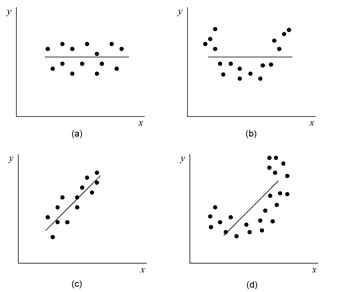
\includegraphics[width=110mm]
        {./figures/scatter.png}}
        %\caption{\label{fig:my-label} My figure.  An example of a cool figure}
      \end{figure}

(a) represents the case where no model exits for the observed data (note: the slope or $\beta_1$ is zero). In this case you would be trying to fit a regression model to noise or random variation. (b) represents the case where the true relationship between $\mathbf{x}$ and $\mathbf{Y}$ is not linear. (c) and (d) represent the case when $H_0: \beta_1 = 0$ is rejected, implying that a model does exist between $\mathbf{x}$ and $\mathbf{Y}$. (c) represents the case where the linear model is sufficient. In the following figure, (d) represents the case where a higher order model may be needed.

First we need to say something about the variance of the estimators. Usually the actual variance $\sigma$ is not known and it is estimated as
\begin{eqnarray}
\hat{\sigma}^2 &=&\dfrac{1}{N-(p+1)}\sum_{i=1}^N(y_i-\hat{y}_i)^2
\end{eqnarray}
Then from \eqref{VarianceEstimatorDiag}, the estimate of the variance of the $j$-th estimator is
\begin{eqnarray}
\text{Var}(\hat{\beta}_j) &\approx& \hat{\sigma}^2 v_j = \hat{\sigma}^2 \left(\mathbf{X}^T\mathbf{X}\right)^{-1}_{jj}\label{VarianceEstimatorDiagEstimate}
\end{eqnarray}
For hypothesis testing, we first calculate the Z-score of the $j$-the estimator
\begin{eqnarray}
z_j &=&\dfrac{\hat{\beta}_j - \beta_j}{\sqrt{\text{Var}(\hat{\beta}_j)}}\nonumber\\
%%
&=&\dfrac{\hat{\beta}_j}{\hat{\sigma} \sqrt{v_j}}
\end{eqnarray}
since $\beta_j = 0$ (the null hypothesis).

Since we do not know the actual variance and we use an estimate of the variance, the appropriate distribution to be used would be the $t$ distribution with $N-(p+1)$ degrees of freedom $t_{N-(p+1)}$ (as opposed to a normal distribution); a large (absolute) value of $z_j$ will lead to rejection of $H_0: \beta_1 = 0$. Note: as the sample size increases, the difference between the tail quantiles of a $t$-distribution and a normal distribution becomes negligible.


\subsection{Confidence Interval or Set}
Recall from \eqref{NormallyDistributedBetaHat} that
\begin{eqnarray}
\boldsymbol{\hat{\beta}}\sim N(\boldsymbol{\beta},\sigma^2 \left(\mathbf{X}^T\mathbf{X}\right)^{-1})
\end{eqnarray}
If one isolates $\beta_j$, we have
\begin{eqnarray}
&&\hat{\beta}_j - \beta_j \sim N(0,\sigma^2 v_j )\:\:\:\:\text{using \eqref{VarianceEstimatorDiag}}\nonumber\\
&\rightarrow&\dfrac{\hat{\beta}_j - \beta_j}{\sigma \sqrt{v_j}} \sim \dfrac{1}{\sigma \sqrt{v_j}}N(0,\sigma^2 v_j )\nonumber\\
&\rightarrow&\dfrac{\hat{\beta}_j - \beta_j}{\sigma \sqrt{v_j}} \sim N(0,1)
\end{eqnarray}
Based on the discussion in Section \ref{SectionChiSquare}, we have
\begin{eqnarray}
&&\left(\dfrac{\hat{\beta}_j - \beta_j}{\sigma \sqrt{v_j}}\right)^2 \sim \chi_1^2\nonumber\\
&\rightarrow&\left(\dfrac{\hat{\beta}_j - \beta_j}{\sqrt{v_j}}\right)^2 \sim \sigma^2\chi_1^2
\end{eqnarray}

\bibliography{databasens}

\end{document} 